\chapter{Systemdesign} % (fold)
\label{sec:systemdesign}
Innerhalb dieses Abschnitt sollen die konkreten Technologien beschrieben werden, die gewählt wurden um ein System zu entwickeln welches für Latentztests verwendet werden kann.
\section{Datenbankdesign} % (fold)
Für die Durchführung des Experiments werden zwei Datenbanktypen verwendet, welche nachfolgend mit ihrer konkreten Konfiguration beschrieben werden.
\label{sec:datenbankdesign}
\subsection{Relationales Datenbankdesign} % (fold)
\label{sec:relationalesdatenbankdesign}

\begin{figure}[H]
	\centering
	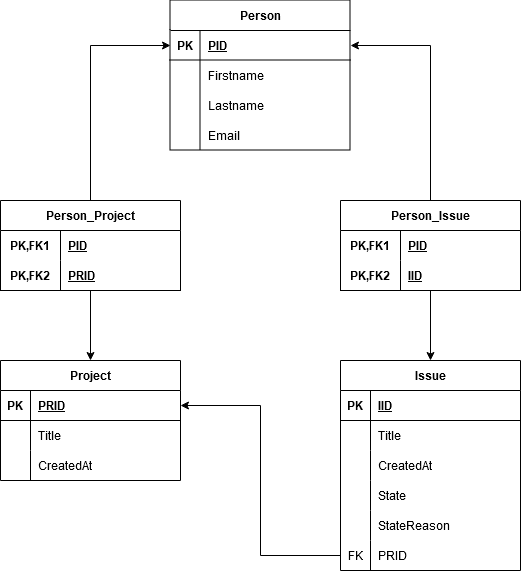
\includegraphics[scale=0.6]{Illustrations/table_diagram.png}
	\caption{Tabellen Diagramm}
\end{figure}
\newpage
\noindent
Um eine relationale Datenbank aus dem gegebenen Datenmodell (Abb. 4.1) zu erstellen muss dieses wie in Abb. 5.1 zu sehen ist angepasst werden, um die Beziehung zwischen Person und Projekt als auch Person und Issue abzubilden. Somit ergeben sich für die relationale Datenbank fünf Tabellen welche in einer PostgreSQL Datenbank realisiert werden. PostgreSQL wird verwendet, da es ein leistungsfähiges, objekt-relationales Datenbanksystem bietet welches Open-Source ist und dadurch kostenfrei zur Verfügung steht. Die Datenbank wurde mit Beispieldaten befüllt, welche in Abbildung 5.2 bis 5.6 beispielhaft zusehen sind. Hierbei wurden 500.000 Personen als auch Projekt und Issue Objekte in die Datenbank eingefügt. Durch die Verwendung von Zwischentabellen, wie person\_issue und person\_project, enthält die relationale Datenbank 2,5 Mio. Tupel, die einen Speicherbedarf von 215MB besitzen.

\begin{figure}[H]
	\centering
	\begin{tabular}{|l | l | l | l |}
	\hline
	pid & firstname & lastname & email \\
	\hline
	1 & Cecilla & Beningfield & cbeningfield9@wp.com \\
	\hline
	\end{tabular}
	\caption{Tupel der Tabelle Person}
\end{figure}
\begin{figure}[H]
	\centering
	\begin{tabular}{|l | l |}
	\hline
	pid & iid \\
	\hline
	1 & 4894 \\
	\hline
	\end{tabular}
	\caption{Tupel der Tabelle Person\_Issue}
\end{figure}
\begin{figure}[H]
	\centering
	\begin{tabular}{|l | l | l | l | l | l|}
	\hline
	iid & title & createdat & state & statereason & prid \\
	\hline
	1 & Dabfeed & 2023-06-10 00:00:00 & Open & Assigned & 586 \\
	\hline
	\end{tabular}
	\caption{Tupel der Tabelle Issue}
\end{figure}
\begin{figure}[H]
	\centering
	\begin{tabular}{|l | l |}
	\hline
	pid & iid \\
	\hline
	1 & 714 \\
	\hline
	\end{tabular}
	\caption{Tupel der Tabelle Person\_Project}
\end{figure}
\begin{figure}[H]
	\centering
	\begin{tabular}{|l | l | l |}
	\hline
	prid & title & createdat \\
	\hline
	1 & Asoka & 2022-02-17 00:00:00 \\
	\hline
	\end{tabular}
	\caption{Tupel der Tabelle Project}
\end{figure}
\newpage


% subsection relationalesdatenbankdesign (end)
\subsection{Graphdatenbankdesign} % (fold)
\label{sec:graphsdatenbankdesign}
Um eine Graphdatenbank zu erstellen benötigt man keine definierten Tabellen, da diese die Daten schemafrei speichert. Die Nodes werden bei der Erstellung entsprechend der Objekte benannt, ebenso werden die Beziehungen zwischen den Nodes bei der Erstellung benannt. Als Graphdatenbank wird auf Neo4j zurückgegriffen. Es ist eine der am weitesten verbreiteten Graphdatenbanken und bietet eine hohe Benutzerfreundlichkeit. In Abbildung 5.7 ist eine Demonstration einer Beziehung zwischen jeweils einem Node zu sehen. Die Kanten sind als gerichtete Kanten abgebildet, dabei hat Person zwei ausgehende Kanten, Projekt zwei eingehende und Issue jeweils eine eingehende als auch eine ausgehende Kante. Wie in der relationalen Datenbank wurden auch in der Graphdatenbank 500.000 Nodes pro Objekt erstellt. Hierbei werden jedoch keine Zwischentabellen benötigt, um Beziehungen darzustellen, wodurch in der Datenbank 1,5 Mio. Nodes vorhanden sind, die durch 2,01 Mio. Edges verbunden sind. Hieraus ergibt sich eine Gesamtgröße von 197MB.


\begin{figure}[H]
	\centering
	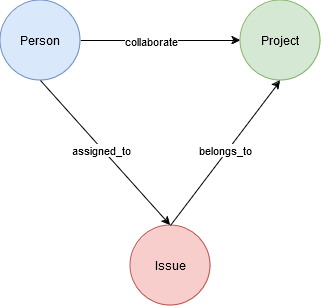
\includegraphics[scale=.8]{Illustrations/graph_diagram}
	\caption{Graph Diagramm}
\end{figure}
% subsection graphdatenbankdesign (end)

% section datenbankdesign (end)
\newpage
\section{Schnittstellendesign} % (fold)
\label{sec:schnittstellendesign}

\subsection{REST}
\label{sec:rest}
Bei REST wird für jedes Testszenario ein seperater Endpunkt benötigt. Hierbei wurden sechs verschiedene Endpunkte mit unterschiedlichen Komplexität entworfen.

\begin{itemize}
\item \textbf{HEAD api/resource} wird verwendet, um einen Head-Request durchzuführen um die Latenz der API zu bestimmen.
\item \textbf{GET api/issues?counter=x\&?joins=y}: Hierbei kann die Menge der Ergebnistupel(x) und die Anzahl der Joins(y) die auf der Datenbank durchgeführt werden bei der Anfrage bestimmt werden. Die in Abbildung 5.8 dargestellte Antwort wird hierbei erwartet.
\begin{figure}[H]
\begin{center}
\begin{BVerbatim}
{
    "pid": 10,
    "firstname": "Cecilla",
    "lastname": "Beningfield",
    "email": "cbeningfield9@wp.com"
}
[...]
\end{BVerbatim}
\end{center}
\caption{GET api/issues?counter=x\&?joins=y Response}
\end{figure}


\item \textbf{GET api/persons/:pid}: Dieser Endpunkt ermöglicht das Abrufen einer bestimmten Person anhand ihrer ID. Die API liefert dabei ein JSON-Objekt zurück, dass die Person mit den Attributen Vorname, Nachname und E-Mail-Adresse beschreibt.(Abb. 5.9)
\begin{figure}[H]
\begin{center}
\begin{BVerbatim}
{
    "pid": 10,
    "firstname": "Cecilla",
    "lastname": "Beningfield",
    "email": "cbeningfield9@wp.com"
}
\end{BVerbatim}
\end{center}
\caption{GET api/persons/:pid Response}
\end{figure}

\item Mit dem Endpunkt  \textbf{GET api/persons} können alle in der Datenbank gespeicherten Personen abgerufen werden. Die Antwort umfasst 5000 Personenobjekte im JSON-Format.(Abb. 5.10)

\begin{figure}[H]
\begin{center}
\begin{BVerbatim}
[
    {
        "pid": 1,
        "firstname": "Ruby",
        "lastname": "Burchatt",
        "email": "rburchatt0@msn.com"
    },
	[...]
    {
        "pid": 5000,
        "firstname": "Murdoch",
        "lastname": "Simonitto",
        "email": "msimonittorr@google.ca"
    }
]
\end{BVerbatim}
\end{center}
\caption{GET api/persons Response}
\end{figure}

\item Der Endpunkt \textbf{GET api/persons/:pid/projects/issue} erhöht die Komplexität, da hier nicht nur auf ein einzelnes Objekt zugegriffen wird. Stattdessen erfordert die Abfrage mehrere Objekte, die miteinander in Abhängigkeit stehen, um die Anfrage zu bearbeiten. Die Antwort umfasst alle Issues die in Projekten vorhanden sind in der eine Person mitwirkt.(Abb. 5.11)
\begin{figure}[H]
\begin{center}
\begin{BVerbatim}
[
   {
        "iid": 1,
        "title": "Pixope",
        "createdAt": "2024-07-23 00:00:00",
        "state": "Closed"
        "stateReason": "Cancelled"
    },
    {
        "iid": 2876,
        "title": "Zoomlounge",
        "createdAt": "2020-08-26 00:00:00",
        "state": "Open"
        "stateReason": "Bug"
    },
]
\end{BVerbatim}
\end{center}
\caption{GET api/persons/:pid/projects/issue Response}
\end{figure}

\item \textbf{POST api/persons/:pid/projects/:prid/issues}: Dieser Endpunkt ermöglicht das Erstellen eines neuen Issues in der Datenbank, um nicht nur Abfragen zu testen, sondern auch das Hinzufügen von Daten. Im Body der Anfrage wird ein Issue-Objekt im JSON-Format übergeben.(Abb. 5.12) 
\newline
\begin{figure}[H]
\begin{center}
\begin{BVerbatim}
{
    "title":"test",
    "createdAt":"2023-02-21T00:00:00",
    "state":"Open",
    "stateReason":"Bug"
}
\end{BVerbatim}
\end{center}
\caption{POST api/persons/:pid/projects/:prid/issues Body}
\end{figure}
Die Antwort enthält das erstellte Issue-Objekt, das eine gültige ID sowie Verknüpfungen zu dem zugehörigen Projekt und der Person beinhaltet.(Abb. 5.13)
\begin{figure}[H]
\begin{center}
\begin{BVerbatim}
{
    "iid": 5207,
    "title": "test",
    "createdAt": "2023-02-21T00:00:00",
    "state": "Open",
    "stateReason": "Bug",
    "project": {
        "prid": 12,
        "title": "Y-find",
        "createdAt": "2021-01-10T00:00:00"
    },
    "assignee"{
        "pid": 1,
        "firstname": "Ruby",
        "lastname": "Burchatt",
        "email": "rburchatt0@msn.com"
    },
}
\end{BVerbatim}
\end{center}
\caption{POST api/persons/:pid/projects/:prid/issues Response}
\end{figure}
\end{itemize}

% section rest (end)

\subsection{GraphQL}
GraphQL unterscheidet sich bei der Art der Anfragen sehr stark zu REST. Es wird nur über den Endpunkt POST api/graphql angesprochen. Hierüber werden sowohl Querys als auch Mutations abgedeckt. Die Anfragen werden im Body mithilfe der GraphQL Query Language definiert, welche JSON sehr ähnlich ist. Die in 5.2.1 definierten REST Endpunkte wurden in GraphQL nachgebildet, sodass sie die selbe Antwort liefern. Für einen HEAD Request bietet GraphQL nativ jedoch keine Lösung, weshalb in GraphQL APIs der HEAD Request identisch wie in den REST APIs implementiert wurde.
Der parametrisierte Endpunkt aus der REST-API wurde in GraphQL wie in Abb. 5.14 dargestellt umgesetzt. Hierbei sind bei Counter Werte zwischen 0 und 1,5 Mio und bei Joins werte zwischen 0 und 3 möglich.

\begin{figure}[H]
\begin{center}
\begin{BVerbatim}
query{
    issuesCount(counter: 10, joins: 1){
	iid
	title 
	createdAt 
	state 
	stateReason
    }
}
\end{BVerbatim}
\end{center}
\caption{GraphQL Query GET api/issues?counter=x\&?joins=y}
\end{figure}
\noindent
Die in Abbildung 5.15 dargestellte Query ist dem REST Enpunkt GET api/persons/:pid eqivalent. Hierbei wird ebenfalls eine ID übergeben, allerdings können die Felder die in der Antwort enthalten sind explizit gewählt werden. Hierbei wurden die Personen ID, Vorname, Nachname als auch die Email gewählt, um die selbe Antwort wie der REST Endpunkt zu erhalten. 
\begin{figure}[H]
\begin{center}
\begin{BVerbatim}
query{
    person(id : 10){
	pid
	firstname
	lastname
	email
    }
}
\end{BVerbatim}
\end{center}
\caption{GraphQL Query equivalent zu GET api/persons/:pid}
\end{figure}
\noindent
Der REST Endpunkt GET api/persons wird von der GraphQL Query in Abbildung 5.16 repräsentiert. Hierbei werden die selben Felder selektiert wie in der vorherigen Abfrage, jedoch wird hierbei die Query persons angesprochen, wodurch alle Personen der Datenbank abgerufen werden.
\begin{figure}[H]
\begin{center}
\begin{BVerbatim}
query {
    persons {
        pid
        firstname
        lastname
        email
    }
}
\end{BVerbatim}
\end{center}
\caption{GraphQL Query equivalent zu GET api/persons}
\end{figure}
\noindent
Abbildung 5.17 zeigt die GraphQL Query, welche dem REST Endpunkt GET api/persons/ :pid/projects/issue entspricht. Hierbei werden die im Schema definierten Querys geschachtelt, um eine Abfrage zu erhalten, welche die Abhängigkeiten zwischen den Objekten repräsentiert.
\begin{figure}[H]
\begin{center}
\begin{BVerbatim}
query{
    person(id : 10){
        projects{
	    issues{
		iid
		title
		createdAt
		state
		stateReason
	    }
        }
    }
}
\end{BVerbatim}
\end{center}
\caption{GraphQL Query equivalent zu GET api/persons/:pid/projects/issue}
\end{figure}
\noindent
Um den REST Endpunkt POST api/persons/:pid/projects/:prid/issues nachzubilden wurde die in Abb. 5.18 dargestellte Mutation entwickelt. Hierbei wird ein Input Objekt definiert, welches die Attribute beinhaltet, die zur Erstellung des Issues benötigt werden. Danach kann, wie auch in den zuvor beschriebenen Querys, selektiert werden, welche Felder in der Antwort enthalten sind.
\begin{figure}[H]
\begin{center}
\begin{BVerbatim}
mutation{
    createIssue(input:{
	title : „Bug in Login“
	createdAt : „2024-12-03T12:30:00
	state : „Open“
	stateReason : „Error in Login“
	prid: 80
	pid: 10
	}){
	iid
	title
	state
	stateReason
	createdAt
    }
}
\end{BVerbatim}
\end{center}
\caption{GraphQL Query equivalent zu POST api/persons/:pid/projects/:prid/issues}
\end{figure}

\label{sec:graphql}
% section graphql (end)

% section schnittstellendesign (end)
\section{Testumgebung} % (fold)
\label{sec:testumgebung}
Zur Ermittlung der Latenzzeiten werden API-Abfragen durchgeführt, bei denen die Antwortzeiten in Millisekunden protokolliert werden. Dafür wird eine Testumgebung mit zwei unterschiedlichen Endgeräten benötigt, um die Last auf mehrere Geräte zu verteilen. Die APIs laufen auf einem Server in Frankfurt, der mit 4 Kernen, 24 GB Arbeitsspeicher, einer 1 Gbit-Internetverbindung und Ubuntu 22.04 als Betriebssystem ausgestattet ist.
\newline
Die Abfragen erfolgen von einem PC mit 8 Kernen, 32 GB Arbeitsspeicher, einer 50 Mbit-Internetverbindung und Windows 10 als Betriebssystem. Die durchschnittliche Latenz (Ping) zwischen Server und PC beträgt 24 ms. Da ein Ping jedoch nur auf ISO Schicht 3 agiert, wird vor jedem Testdurchlauf mithilfe von HEAD-Requests, die in 5.2.1 beschrieben wurden, eine Latenz zwischen den Endgeräten ermittelt die alle ISO-Schichten durchläuft. Um Schwankungen in der Netzwerkauslastung und der Systembelastung zu minimieren, werden pro Testszenario und API jeweils 100 Anfragen ausgeführt. Insgesamt ergibt dies bei 4 APIs und 25 Testszenarien eine Datengrundlage von 10.000 Latenzzeiten.


% section testumgebung (end)


% chapter Systemdesign (end)